
\ifnum \Version=1
% FOR 14.2
\question[4] Show that the function does not have a limit as $(x,y) \to (1,0)$.  
    \begin{align}
        f(x,y) = \frac{xy^2 - y^2}{(x-1)^2 +y^4}
    \end{align}
\ifnum \Solutions=1 {\color{DarkBlue} \\ \textit{Solutions:} The path $x=ky^2+1$ passes through the point $(1,0)$. We can evaluate the limit along this path. 
    \begin{align}
        f(x,y) &= \frac{xy^2 - y^2}{(x-1)^2 +y^4} \\
        f(ky^2+1,y) 
        &= \frac{(ky^2+1)y^2 - y^2}{((ky^2+1)-1)^2 +y^4} \\
        &= \frac{ky^4+ y^2 - y^2}{(ky^2 + 0 )^2 +y^4} \\
        &= \frac{k^2y^4}{ky^4 +y^4} \\
        &= \frac{k}{k^2+1}
    \end{align}
    The result depends on $k$ and therefore the limit does not exist. 

    } 
   \else
      
   \fi
    
\fi











% SECTION 14.7 
\ifnum \Version=2
% VERBATUM FROM SPRING 2022
\question[6] Identify the locations of all of the critical points of $f(x,y) = x^4+y^4-4xy$ and classify the critical points using the second derivative test. Please show your work. 

\ifnum \Solutions=1 {\color{DarkBlue} \textit{Solutions:} Setting $\nabla f = \langle 4x^3-4y, 4y^3-4x\rangle = \mathbf 0 = \langle 0,0\rangle$. The first entries give $y=x^3$, and substituting this into the second entries yields $$4(x^3)^3 -4x = 0 \quad \Rightarrow \quad  x(x^8-1) = 0$$
So $\nabla f =0$ for $x = 0, + 1, -1$. So if $y=x^3$ the critical points are: $(0,0), (-1,-1), (1,1)$. The second derivatives of $f$ are
$$f_{xx} = 12x^2, \quad f_{yy} = 12y^2, \quad f_{xy} = -4$$
The function we need for the second derivative test is 
$$D(x,y) = (12x^2)(12y^2) - (-4)^2$$
At $(1,1)$, $D>0$, and $f_{xx}>0$, so the point is a \textbf{minimum}.  \\
At $(-1,-1)$, $D>0$, and $f_{xx}>0$, so the point is a \textbf{minimum}.  \\
At $(0,0)$, $D<0$, so the point is a \textbf{saddle}.  
} 
\else
\fi    
\fi



\ifnum \Version=3
% DIFFERENTIALS AND GRADIENTS
\question[6] Suppose $f(x,y,z) = 6x^2+3y^2+3z$. 

\begin{parts}
    \part Use the differential $df$ to estimate how much $f(x,y,z)$ will change if the point $P(x,y,z)$ moves from $P_0(2,1,3)$ a distance of $ds = 1/10$ in the direction of $\mathbf v = 2\mathbf i + \mathbf j + 2\mathbf k$. Please show your work. 
    \ifnum \Solutions=1 {\color{DarkBlue} \\ \textit{Solutions:} 
    The gradient of $f$ at $P_0$ is
    \begin{align}
        \nabla f &= \begin{pmatrix} 12x\\6y\\3\end{pmatrix} 
        \quad \Rightarrow \quad 
        \nabla f(2,1,3) = \begin{pmatrix} 24\\6\\3\end{pmatrix} 
    \end{align}
    A unit vector in the direction of $\mathbf v$ is
    \begin{align}
        \mathbf u = \frac{\mathbf v}{|\mathbf v|} = \begin{pmatrix} 2/3\\1/3\\2/3 \end{pmatrix}
    \end{align}
    The differential $df$ at $P_0$ is
    \begin{align}
        df = \nabla f \cdot \mathbf u \, ds &= \begin{pmatrix} 24\\6\\3\end{pmatrix}   \cdot \begin{pmatrix} 2/3\\1/3\\2/3 \end{pmatrix} ds 
        = (24\cdot 2/3 + 6 \cdot 1/3 + 3 \cdot 2/3) ds = 20ds
    \end{align}
    If $ds = 1/10$ then $df = 2$. 
    }
    \else
    \vspace{7cm}
    \fi
    \part NEED TO FIX THIS PROBLEM - THE POINT ISN'T ON THE SURFACE AND Construct parametric equations for the line that is tangent to the curve of intersection of $f(x,y,z)=1$ and the surface $g(x,y,z) = x+y+z - 3 = 0$ at the point $Q(1,1,1)$. You can use your results from part (a), and please show your work. 
    \ifnum \Solutions=1 {\color{DarkBlue} \\ \textit{Solutions:} The tangent line is orthogonal to both $\nabla f$ and $\nabla g$ at $Q$, and therefore parallel to $\mathbf v = \nabla f \times \nabla g$. 
    \begin{align}
        \nabla f &= \begin{pmatrix} 12x\\6y\\3\end{pmatrix} \quad \Rightarrow \quad 
        \nabla f(1,1,1) = \begin{pmatrix} 12\\6\\3\end{pmatrix} \\
        \nabla g &= \begin{pmatrix} 1\\1\\1\end{pmatrix} \quad \Rightarrow \quad 
        \nabla g(1,1,1) = \begin{pmatrix} 1\\1\\1\end{pmatrix} \\
        \nabla f \times \nabla g &= \begin{vmatrix} \mathbf i & \mathbf j & \mathbf k \\ 12&6&3\\1&1&1\end{vmatrix} = \begin{pmatrix} 3\\-9\\6 \end{pmatrix}
    \end{align}
    The parametric equations for the tangent line at $Q$ have the form $\mathbf x = \mathbf x_0 + t\mathbf v$. Therefore,
    \begin{align}
        \mathbf x &= \begin{pmatrix}1\\1\\1 \end{pmatrix} + t\begin{pmatrix} 3\\-9\\6 \end{pmatrix}
    \end{align}
    We could also express the parametric equations for the tangent line by listing out each of the components of vector $\mathbf x$. 
    } 
    \else 
    
    \fi
\end{parts}


\fi







% SECTION 14.7 
\ifnum \Version=4
\question[6] Consider the function $\displaystyle f(x,y) = \frac12x^2+\frac14y^4-xy$. 
\begin{parts}
    \part Identify all of the critical points of $f(x,y)$. Please show your work. 
    
    \ifnum \Solutions=1 {\color{DarkBlue} \textit{Solutions:} Setting $\nabla f = \langle x-y, y^3-x\rangle = \mathbf 0 = \langle 0,0\rangle$ yields
    \begin{align}
        x-y &= 0, \quad \Rightarrow\quad y = x\\
        y^3-x &=0 , \quad \Rightarrow\quad x=y^3
    \end{align}
    Eliminating $x$ gives us
    \begin{align}
        y &= y^3 \quad \Rightarrow \quad y = 0, \pm 1
    \end{align}
    Substituting into the first component of the gradient equation gives us three points. The only critical points are $(0,0)$, $(-1,-1)$, and $(1,1)$.
    } 
    \else
    \vspace{6cm}
    \fi    
    \part Classify the critical points using the second derivative test, if possible. Please show your work. You may use your results from part (a). 
    
    \ifnum \Solutions=1 {\color{DarkBlue}
    The second derivatives of $f$ are
    $$f_{xx} = 1, \quad f_{yy} = 3y^2, \quad f_{xy} = -1$$
    The function we need for the second derivative test is 
    $$D(x,y) = (1)(3y^2) - (-1)^2 = 3y^2 -1$$
    At $(-1,-1)$, $D=2>0$, and $f_{xx}>0$, so the point is a \textbf{minimum}.  \\
    At $(0,0)$, $D=-1<0$, so the point is a \textbf{saddle}.  \\
    At $(1,1)$, $D=2>0$, and $f_{xx}>0$, so the point is a \textbf{minimum}.  \\
    } 
    \else 
    \vspace{2 cm}
    \fi
\end{parts}
\fi

\ifnum \Version=5
% DIFFERENTIALS AND GRADIENTS
\question[6] Suppose $f(x,y,z) = 2x^3+5y^3+10z$. 

\begin{parts}
    \part Use the differential $df$ to estimate how much $f(x,y,z)$ will change if the point $P(x,y,z)$ moves from $P_0(2,2,1)$ a distance of $ds = 0.1$ in the direction of $\mathbf v = \langle 0,4,3 \rangle$. Please show your work. 
    \ifnum \Solutions=1 {\color{DarkBlue} \\ \textit{Solutions:} 
    The gradient of $f$ at $P_0$ is
    \begin{align}
        \nabla f &= \begin{pmatrix} 6x^2\\15y^2\\10\end{pmatrix} 
        \quad \Rightarrow \quad 
        \nabla f(2,2,1) = \begin{pmatrix} 24\\60\\10\end{pmatrix} 
    \end{align}
    A unit vector in the direction of $\mathbf v$ is
    \begin{align}
        \mathbf u = \frac{\mathbf v}{|\mathbf v|} = \begin{pmatrix} 0\\4/5\\3/5 \end{pmatrix}
    \end{align}
    The differential $df$ at $P_0$ is
    \begin{align}
        df = \nabla f \cdot \mathbf u \, ds 
        &= \begin{pmatrix} 24\\60\\10\end{pmatrix} \cdot \begin{pmatrix} 0\\4/5\\3/5 \end{pmatrix} ds 
        = (24\cdot 0 + 60 \cdot 4/5 + 10 \cdot 3/5) ds = (48+6)ds
    \end{align}
    If $ds = 1/10$ then $df = 5.4$ or $df = \frac{54}{10}=\frac{27}{5}$.
    }
    \else
    \vspace{7cm}
    \fi
    \part Construct the equation to the tangent plane to the surface $f(x,y,z) = 2x^3+5y^3+10z = 42$ at the point $P_0(2,2,1)$. Please show your work. You can use your work from part (a). 
    \ifnum \Solutions=1 {\color{DarkBlue} \\ \textit{Solutions:} A vector normal to the tangent plane at $P_0$ is 
    \begin{align}
        \nabla f &= \begin{pmatrix} 6x^2\\15y^2\\10\end{pmatrix} 
        \quad \Rightarrow \quad 
        \nabla f(2,2,1) = \begin{pmatrix} 24\\60\\10\end{pmatrix} 
    \end{align}
    A point on the plane is $P_0(2,2,1)$. The plane has the equation
    \begin{align}
        0 &= \mathbf n \cdot (\mathbf x - \mathbf x_0) = 24(x-2) + 60(y-2) + 10(z-1)
    \end{align}
    It isn't necessary to simplify further, but we could rearrange the equation to any of the forms below. 
    \begin{align}
        24(x-2) + 60(y-2) + 10(z-1) &= 0 \\
        24x+60y+10z &= 178 \\
        12x+30y+5z &= 89
    \end{align}
    } 
    \else 
    
    \fi
\end{parts}
\fi



% SECTION 14.7 
\ifnum \Version=6
\question[6] Consider the function $\displaystyle f(x,y) = \frac12x^2+\frac13y^3-xy$. 
\begin{parts}
    \part Identify all of the critical points of $f(x,y)$. Please show your work. 
    
    \ifnum \Solutions=1 {\color{DarkBlue} \textit{Solutions:} Setting $\nabla f = \langle x-y, y^2-x\rangle = \mathbf 0 = \langle 0,0\rangle$ yields
    \begin{align}
        x-y &= 0, \quad \Rightarrow\quad y = x\\
        y^2-x &=0 , \quad \Rightarrow\quad x=y^2
    \end{align}
    Eliminating $x$ gives us $y = y^2 \ \Rightarrow \ y = 0, 1$. 
    Substituting into the first component of the gradient equation gives us two points. The only critical points are $(0,0)$ and $(1,1)$.
    } 
    \else
    \vspace{3cm}
    \fi    
    
    \part Identify the absolute maximum and absolute minimum values of $f(x,y)$ on the plate bounded by $x=0$, $y=0$, and $y=5-x$. Identify where these extrema are located. Please show your work. You may use your results from part (a). 
    
    \ifnum \Solutions=1 {\color{DarkBlue}
    Boundaries:
    \begin{itemize}
        \item Along $x=0$ and $0\le y \le 5$, $f(0,y) = \frac13y^3$, minimum at $(0,0)$ and maximum at $(0,5)$. 
        \item Along $y=0$ and $0\le x \le 5$, $f(x,0) = \frac12x^2$, minimum at $(0,0)$ and maximum at $(5,0)$. 
        \item Along $y=5-x$ and $0\le x \le 5$, we obtain \begin{align}
            f(x,5-x) &= \frac12x^2 +\frac13(5-x)^3-x(5-x) \\
            &= \frac12x^2+\frac13(5-x)^3-5x+x^2\\
            \frac{d}{dx}f(x,5-x) &= x-(5-x)^2-5+2x \\
            &= 3x-(x^2-10x+25)-5 \\
            &= -x^2 + 13x-30 \\
            &= -(x-3)(x-10)
        \end{align}
        Critical points at $x=3$ and $x=10$, but we can ignore $x=10$. Possible min and max: 
        \begin{align}
            f(0,0) &= 0 \\
            f(1,1) &= \frac12+\frac13-1 = -1/6 \\
            f(0,5) &= 125/3 \\
            f(5,0) &= 25/2 \\ 
            f(3,2) &= \frac92 + \frac83 - 6 = \frac{43}{6} - \frac{36}{6} = \frac{7}{6}
        \end{align}
        The absolute min is $f(1,1)=-\frac16$, the absolute max is $f(0,5) = 125/3$. 
    \end{itemize}
    
    } 
    \else 
    \vspace{2 cm}
    \fi
\end{parts}
\fi






% SECTION 14.7 
\ifnum \Version=7
\question[6] Consider the function $\displaystyle f(x,y) = x^2+y^4-4xy$. 
\begin{parts}
    \part Identify all of the critical points of $f(x,y)$. Please show your work. 
    
    \ifnum \Solutions=1 {\color{DarkBlue} \textit{Solutions:} Setting $\nabla f = \mathbf 0 = \langle 0,0\rangle$ yields
    \begin{align}
        \DFDX = 2x-4y &= 0, \quad \Rightarrow\quad x = 2y\\
        \DFDY = 4y^3-4x &=0 , \quad \Rightarrow\quad x=y^3
    \end{align}
    Eliminating $x$ gives us
    \begin{align}
        0 &= y^3 - 2y \\
        0 &= y(y^2-2) \quad \Rightarrow \quad y = 0, \pm \sqrt2
    \end{align}
    Substituting into the first component of the gradient equation gives us three points. 
    \begin{align}
        y = 0 \ &\Rightarrow \ x = 2\cdot0 \ \Rightarrow (0,0) \\
        y = \sqrt2 \ &\Rightarrow \ x = 2\sqrt 2 \ \Rightarrow (2\sqrt2,\sqrt2) \\
        y = -\sqrt2 \ &\Rightarrow \ x = -2\sqrt 2 \ \Rightarrow (-2\sqrt2,-\sqrt2) 
    \end{align}
    } 
    \else
    \vspace{6cm}
    \fi    
    \part Classify the critical points using the second derivative test, if possible. Please show your work. You may use your results from part (a). 
    
    \ifnum \Solutions=1 {\color{DarkBlue}
    The second derivatives of $f$ are
    \begin{align}
            f_{xx} &= \DDX (2x-4y) = 2 \\
            f_{yy} &= \DDY (4y^3-4x) = 12y^2 \\
            f_{xy} &= \DDX (4y^3-4x) = -4
    \end{align}
    The function we need for the second derivative test is 
    $$D(x,y) = f_{xx}f_{yy} - (f_{xy})^2 = (2)(12y^2) - (-4)^2 = 24y^2 - 16$$
    Evaluate at each critical point: 
    \begin{itemize}
        \item At $(0,0)$, $D=-16<0$, so the point is a \textbf{saddle}.
        \item At $(2\sqrt2,2)$, $D>0$, and $f_{xx}>0$, so the point is a \textbf{minimum}.
        \item At $(-2\sqrt2,-2)$, $D>0$, and $f_{xx}>0$, so the point is a \textbf{minimum}.
    \end{itemize}
    Please note the following. 
    \begin{itemize}
        \item It isn't necessary to work out \textbf{exactly} what $D$ is equal to, because we only need to determine if $D$ is positive, negative, or zero. So if a student were to get the incorrect value of $D$, we don't actually need to deduct points for that error, unless the error led to a mistake in determining whether $D$ were positive, negative, or zero. 
        \item Some students listed the points $(2\sqrt2,-\sqrt2)$ or at $(-2\sqrt2,\sqrt2)$ as critical points in part (a). But there isn't a critical point at $(2\sqrt2,-\sqrt2)$ or at $(-2\sqrt2,\sqrt2)$ because we found that $x=2y$. In other words, $x$ and $y$ must have the same sign. 
        \item The second derivative test is given by the following. 

        \begin{center}\begin{tikzpicture} \node [mybox](box){\begin{minipage}{0.75\textwidth}\vspace{4pt}
    Let \( f(x, y) \) be a function of two variables with continuous second partial derivatives in a neighborhood of a point \( (a, b) \), and $f_x(a,b) = f_y(a,b) = 0$. Suppose also that $D$ is the \textbf{discriminant} $$D = f_{xx}(a, b) \cdot f_{yy}(a, b) - [f_{xy}(a, b)]^2 $$
    Then we can classify the critical point $(a,b)$ as follows. 
    \vspace{4pt}
    \begin{itemize}
        \item If \( D > 0 \) and \( f_{xx}(a, b) > 0 \), then \( f \) has a local minimum at \( (a, b) \).
        \item If \( D > 0 \) and \( f_{xx}(a, b) < 0 \), then \( f \) has a local maximum at \( (a, b) \).
        \item If \( D < 0 \), then \( f \) has a saddle point at \( (a, b) \).
        \item If \( D = 0 \), the test is inconclusive.
    \end{itemize}    
    \vspace{2pt}
    \end{minipage}};
    \node[fancytitle, right=10pt] at (box.north west) {Second Derivative Test};
    \end{tikzpicture} \end{center} 
    Note that the discriminant \( D \) helps determine the \textbf{concavity} of the function at the critical point. If \( D > 0 \), it indicates that the graph is either concave up or concave down. The sign of \( f_{xx}(a, b) \) then determines whether the critical point is a local minimum or local maximum. And it is important to note that the second derivative test only provides information about local extrema; it does not reveal information about global extrema or points where the function may not have a derivative.

    \end{itemize}
    } 
    \else 
    \vspace{2 cm}
    \fi
    % \part Determine the absolute minimum value of $f(x,y)$, and all locations where this value is obtained.
\end{parts}
\fi





\ifnum \Version=8
% DIFFERENTIALS AND GRADIENTS
\question[6] Suppose $f(x,y,z) = x^3+y^2+z^5$. 

\begin{parts}
    \part Use the differential $df$ to estimate how much $f(x,y,z)$ will change if the point $P(x,y,z)$ moves from $P_0(0,1,1)$ a distance of $ds = 0.1$ in the direction of $\mathbf v = \langle 4,0,3 \rangle$. Please show your work. 
    \ifnum \Solutions=1 {\color{DarkBlue} \\ \textit{Solutions:} 
    The gradient of $f$ at $P_0$ is
    \begin{align}
        \nabla f &= \begin{pmatrix} 3x^2\\2y\\5z^4\end{pmatrix} 
        \quad \Rightarrow \quad 
        \nabla f(0,1,1) = \begin{pmatrix} 0\\2\\5\end{pmatrix} 
    \end{align}
    A unit vector in the direction of $\mathbf v$ is
    \begin{align}
        \mathbf u = \frac{\mathbf v}{|\mathbf v|} = \begin{pmatrix} 4/5\\0\\3/5 \end{pmatrix}
    \end{align}
    The differential $df$ at $P_0$ is
    \begin{align}
        df = \nabla f \cdot \mathbf u \, ds 
        &= \begin{pmatrix} 0\\2\\5\end{pmatrix} \cdot \begin{pmatrix} 4/5\\0\\3/5 \end{pmatrix} ds 
        = 3\,ds
    \end{align}
    If $ds = 1/10$ then $df = 3/10$ or $df = 0.3$.
    }
    \else
    \vspace{7cm}
    \fi
    \part Construct the equation to the tangent plane to the surface $f(x,y,z) = x^3+y^2+z^5 = 2$ at the point $P_0(0,1,1)$. Please show your work. You can use your work from part (a). 
    \ifnum \Solutions=1 {\color{DarkBlue} \\ \textit{Solutions:} A vector normal to the tangent plane at $P_0$ is 
    \begin{align}
        \nabla f &= \begin{pmatrix} 3x^2\\2y\\5z^4\end{pmatrix} 
        \quad \Rightarrow \quad 
        \nabla f(0,1,1) = \begin{pmatrix} 0\\2\\5\end{pmatrix} 
    \end{align}
    A point on the plane is $P_0(0,1,1)$. The plane has the equation
    \begin{align}
        0 &= \mathbf n \cdot (\mathbf x - \mathbf x_0) = 0(x-0) + 2(y-1) + 5(z-1)
    \end{align}
    It isn't necessary to simplify further, but we could rearrange the equation to another form. 
    } 
    \else 
    
    \fi
\end{parts}
\fi



\ifnum \Version=9
% DIFFERENTIALS AND GRADIENTS
\question[6] Suppose $f(x,y,z) = x^3+y^2+3z^4$. 

\begin{parts}
    \part Use the differential $df$ to estimate how much $f(x,y,z)$ will change if the point $P(x,y,z)$ moves from $P_0(2,0,1)$ a distance of $ds = 0.2$ in the direction of $\mathbf v = \langle 1,2,2 \rangle$. Please show your work. 
    \ifnum \Solutions=1 {\color{DarkBlue} \\ \textit{Solutions:} 
    The gradient of $f$ at $P_0$ is
    \begin{align}
        \nabla f &= \begin{pmatrix} 3x^2\\2y\\12z^3\end{pmatrix} 
        \quad \Rightarrow \quad 
        \nabla f(2,0,1) = \begin{pmatrix} 12\\0\\12\end{pmatrix} 
    \end{align}
    A unit vector in the direction of $\mathbf v$ is
    \begin{align}
        \mathbf u = \frac{\mathbf v}{|\mathbf v|} = \begin{pmatrix} 1/3\\2/3\\2/3 \end{pmatrix}
    \end{align}
    The differential $df$ at $P_0$ is
    \begin{align}
        df = \nabla f \cdot \mathbf u \, ds 
        &= \begin{pmatrix} 12\\0\\12\end{pmatrix} \cdot \begin{pmatrix}  1/3\\2/3\\2/3  \end{pmatrix} ds 
        = 12\,ds
    \end{align}
    If $ds = 2/10$ then $df = 12\cdot 2/10$ or $df = 2.4$.
    }
    \else
    \vspace{7cm}
    \fi
    \part Construct the equation to the tangent plane to the surface $f(x,y,z) = x^3+y^2+3z^4 = 11$ at the point $P_0(2,0,1)$. Please show your work. You can use your work from part (a). 
    \ifnum \Solutions=1 {\color{DarkBlue} \\ \textit{Solutions:} A vector normal to the tangent plane at $P_0$ is 
    \begin{align}
        \nabla f &= \begin{pmatrix} 3x^2\\2y\\12z^3\end{pmatrix} 
        \quad \Rightarrow \quad 
        \nabla f(2,0,1) = \begin{pmatrix} 12\\0\\12\end{pmatrix} 
    \end{align}
    A point on the plane is $P_0(2,0,1)$. The plane has the equation
    \begin{align}
        0 &= \mathbf n \cdot (\mathbf x - \mathbf x_0) = 12(x-2) + 0(y-0) + 12(z-1)
    \end{align}
    It isn't necessary to simplify further, but we could rearrange the equation to another form. We could, for example, express this as
    $$x+z = 3$$
    However, it would be incorrect to express the answer as
    $$12(x-2) + 0(y-0) + 12(z-1)$$
    The question asked for an equation, so we should give an equation. 
    } 
    \else 
    
    \fi
\end{parts}
\fi




\ifnum \Version=10
% DIFFERENTIALS AND GRADIENTS
\question[6] Suppose $f(x,y,z) = x^3+y^2+z^5$. 

\begin{parts}
    \part Use the differential $df$ to estimate how much $f(x,y,z)$ will change if the point $P(x,y,z)$ moves from $P_0(0,1,1)$ a distance of $ds = 0.1$ in the direction of $\mathbf v = \langle 4,0,3 \rangle$. Please show your work. 
    \ifnum \Solutions=1 {\color{DarkBlue} \\ \textit{Solutions:} 
    The gradient of $f$ at $P_0$ is
    \begin{align}
        \nabla f &= \begin{pmatrix} 3x^2\\2y\\5z^4\end{pmatrix} 
        \quad \Rightarrow \quad 
        \nabla f(0,1,1) = \begin{pmatrix} 0\\2\\5\end{pmatrix} 
    \end{align}
    A unit vector in the direction of $\mathbf v$ is
    \begin{align}
        \mathbf u = \frac{\mathbf v}{|\mathbf v|} = \begin{pmatrix} 4/5\\0\\3/5 \end{pmatrix}
    \end{align}
    The differential $df$ at $P_0$ is
    \begin{align}
        df = \nabla f \cdot \mathbf u \, ds 
        &= \begin{pmatrix} 0\\2\\5\end{pmatrix} \cdot \begin{pmatrix} 4/5\\0\\3/5 \end{pmatrix} ds 
        = 3\,ds
    \end{align}
    If $ds = 1/10$ then $df = 3/10$ or $df = 0.3$.
    }
    \else
    \vspace{7cm}
    \fi
    \part Construct the equation to the tangent plane to the surface $f(x,y,z) = x^3+y^2+z^5 = 2$ at the point $P_0(0,1,1)$. Please show your work. You can use your work from part (a). 
    \ifnum \Solutions=1 {\color{DarkBlue} \\ \textit{Solutions:} A vector normal to the tangent plane at $P_0$ is 
    \begin{align}
        \nabla f &= \begin{pmatrix} 3x^2\\2y\\5z^4\end{pmatrix} 
        \quad \Rightarrow \quad 
        \nabla f(0,1,1) = \begin{pmatrix} 0\\2\\5\end{pmatrix} 
    \end{align}
    A point on the plane is $P_0(0,1,1)$. The plane has the equation
    \begin{align}
        0 &= \mathbf n \cdot (\mathbf x - \mathbf x_0) = 0(x-0) + 2(y-1) + 5(z-1)
    \end{align}
    It isn't necessary to simplify further, but we could rearrange the equation to another form. We could, for example, express this as
    $$2y+5z = 7$$
    However, it would be incorrect to express the answer as
    $$2(y-1) + 5(z-1)$$
    The question asked for an equation, so we should give an equation. 
    } 
    \else 
    
    \fi
\end{parts}
\fi

% SECTION 14.7 
\ifnum \Version=100
\question[6] Consider the function $\displaystyle f(x,y) = \frac12x^2+\frac13y^3-xy+x-y$. WORKING ON THIS PART B NOT FINISHED
\begin{parts}
    \part Identify all of the critical points of $f(x,y)$. Please show your work. 
    
    \ifnum \Solutions=1 {\color{DarkBlue} \textit{Solutions:} Setting $\nabla f = \langle x-y, y^2-x\rangle = \mathbf 0 = \langle 0,0\rangle$ yields
    \begin{align}
        x-y + 1 &= 0 \quad \Rightarrow\quad x = y - 1\\
        y^2-x - 1&=0  \quad \Rightarrow\quad x=y^2 - 1
    \end{align}
    Adding the two gives us 
    \begin{align}
        0 &= y^2 - y = y(y -1)
    \end{align} Thus $y = 0, 1$. Then substituting into the first component of the gradient equation gives us the two points. The only critical points are $(-1,0)$ and $(0,1)$. It isn't necessary to sketch the curves but if we did we can see where the two curves intersect. The intersection points are the critical points. 
    \begin{center}     
    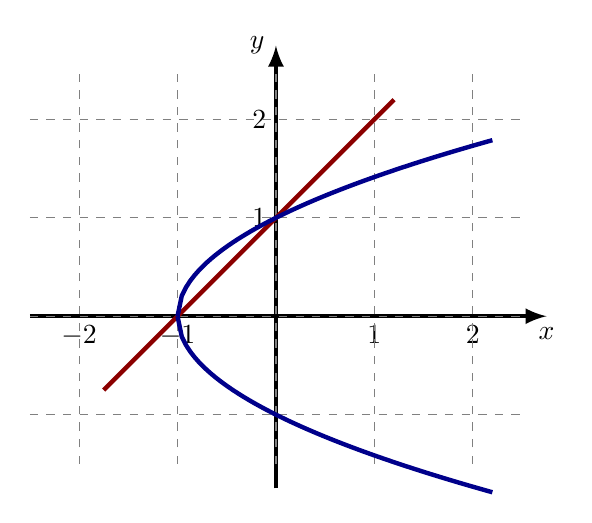
\begin{tikzpicture}[scale=1.25]
      \draw[ultra thick,->,>=latex] (-2.5,0)--(2.75,0) node[below] {$x$};
      \draw[ultra thick,->,>=latex] (0,-1.75)--(0,2.75) node[left] {$y$};
      \draw (0,1) node[left] {$1$};  
      \draw (0,2) node[left] {$2$};      
      \draw (-1,0) node[below] {$-1$};          
      \draw (-2,0) node[below] {$-2$};          
      \draw (1,0) node[below] {$1$};
      \draw (2,0) node[below] {$2$};
      \draw[help lines,gray,thin,dashed] (-2.5, -1.5) grid (2.5, 2.5);
      \draw[domain=-1.75:1.2,ultra thick,samples=75,DarkRed] plot ({\x},{\x+1});
      \draw[domain=-1:2.2,ultra thick,samples=75,DarkBlue] plot ({\x},{sqrt(\x+1)});
      \draw[domain=-1:2.2,ultra thick,samples=75,DarkBlue] plot ({\x},{-sqrt(\x+1)});
    \end{tikzpicture}
    \end{center}      
    } 
    \else
    \vspace{3cm}
    \fi    
    
    \part Identify the absolute maximum and absolute minimum values of $f(x,y)$ on the plate bounded by $x=0$, $y=0$, and $y=5-x$. Identify where these extrema are located. Please show your work. You may use your results from part (a). 
    
    \ifnum \Solutions=1 {\color{DarkBlue}
    Boundaries:
    \begin{itemize}
        \item Along $x=0$ and $0\le y \le 5$, $f(0,y) = \frac13y^3$, minimum at $(0,0)$ and maximum at $(0,5)$. 
        \item Along $y=0$ and $0\le x \le 5$, $f(x,0) = \frac12x^2$, minimum at $(0,0)$ and maximum at $(5,0)$. 
        \item Along $y=5-x$ and $0\le x \le 5$, we obtain \begin{align}
            f(x,5-x) &= \frac12x^2 +\frac13(5-x)^3-x(5-x) \\
            &= \frac12x^2+\frac13(5-x)^3-5x+x^2\\
            \frac{d}{dx}f(x,5-x) &= x-(5-x)^2-5+2x \\
            &= 3x-(x^2-10x+25)-5 \\
            &= -x^2 + 13x-30 \\
            &= -(x-3)(x-10)
        \end{align}
        Critical points at $x=3$ and $x=10$, but we can ignore $x=10$. Possible min and max: 
        \begin{align}
            f(0,0) &= 0 \\
            f(1,1) &= \frac12+\frac13-1 = -1/6 \\
            f(0,5) &= 125/3 \\
            f(5,0) &= 25/2 \\ 
            f(3,2) &= \frac92 + \frac83 - 6 = \frac{43}{6} - \frac{36}{6} = \frac{7}{6}
        \end{align}
        The absolute min is $f(1,1)=-\frac16$, the absolute max is $f(0,5) = 125/3$. 
    \end{itemize}
    
    } 
    \else 
    \vspace{2 cm}
    \fi
\end{parts}
\fi






% SECTION 14.7 
\ifnum \Version=11
\question[6] Consider the function $\displaystyle f(x,y) = x^2+y^4-4xy$. 
\begin{parts}
    \part Identify all of the critical points of $f(x,y)$. Please show your work. 
    
    \ifnum \Solutions=1 {\color{DarkBlue} \textit{Solutions:} Setting $\nabla f = \mathbf 0 = \langle 0,0\rangle$ yields
    \begin{align}
        \DFDX = 2x-4y &= 0, \quad \Rightarrow\quad x = 2y\\
        \DFDY = 4y^3-4x &=0 , \quad \Rightarrow\quad x=y^3
    \end{align}
    Eliminating $x$ gives us
    \begin{align}
        0 &= y^3 - 2y \\
        0 &= y(y^2-2) \quad \Rightarrow \quad y = 0, \pm \sqrt2
    \end{align}
    Substituting into the first component of the gradient equation gives us three points. 
    \begin{align}
        y = 0 \ &\Rightarrow \ x = 2\cdot0 \ \Rightarrow (0,0) \\
        y = \sqrt2 \ &\Rightarrow \ x = 2\sqrt 2 \ \Rightarrow (2\sqrt2,\sqrt2) \\
        y = -\sqrt2 \ &\Rightarrow \ x = -2\sqrt 2 \ \Rightarrow (-2\sqrt2,-\sqrt2) 
    \end{align}
    } 
    \else
    \vspace{6cm}
    \fi    
    \part Classify the critical points using the second derivative test, if possible. Please show your work. You may use your results from part (a). 
    
    \ifnum \Solutions=1 {\color{DarkBlue}
    The second derivatives of $f$ are
    \begin{align}
            f_{xx} &= \DDX (2x-4y) = 2 \\
            f_{yy} &= \DDY (4y^3-4x) = 12y^2 \\
            f_{xy} &= \DDX (4y^3-4x) = -4
    \end{align}
    The function we need for the second derivative test is 
    $$D(x,y) = f_{xx}f_{yy} - (f_{xy})^2 = (2)(12y^2) - (-4)^2 = 24y^2 - 16$$
    Evaluate at each critical point: 
    \begin{itemize}
        \item At $(0,0)$, $D=-16<0$, so the point is a \textbf{saddle}.
        \item At $(2\sqrt2,2)$, $D>0$, and $f_{xx}>0$, so the point is a \textbf{minimum}.
        \item At $(-2\sqrt2,-2)$, $D>0$, and $f_{xx}>0$, so the point is a \textbf{minimum}.
    \end{itemize}
    Please note the following. 
    \begin{itemize}
        \item It isn't necessary to work out \textbf{exactly} what $D$ is equal to, because we only need to determine if $D$ is positive, negative, or zero. So if a student were to get the incorrect value of $D$, we don't actually need to deduct points for that error, unless the error led to a mistake in determining whether $D$ were positive, negative, or zero. 
        \item Some students listed the points $(2\sqrt2,-\sqrt2)$ or at $(-2\sqrt2,\sqrt2)$ as critical points in part (a). But there isn't a critical point at $(2\sqrt2,-\sqrt2)$ or at $(-2\sqrt2,\sqrt2)$ because we found that $x=2y$. In other words, $x$ and $y$ must have the same sign. 
        \item The second derivative test is given by the following. 

        \begin{center}\begin{tikzpicture} \node [mybox](box){\begin{minipage}{0.75\textwidth}\vspace{4pt}
    Let \( f(x, y) \) be a function of two variables with continuous second partial derivatives in a neighborhood of a point \( (a, b) \), and $f_x(a,b) = f_y(a,b) = 0$. Suppose also that $D$ is the \textbf{discriminant} $$D = f_{xx}(a, b) \cdot f_{yy}(a, b) - [f_{xy}(a, b)]^2 $$
    Then we can classify the critical point $(a,b)$ as follows. 
    \vspace{4pt}
    \begin{itemize}
        \item If \( D > 0 \) and \( f_{xx}(a, b) > 0 \), then \( f \) has a local minimum at \( (a, b) \).
        \item If \( D > 0 \) and \( f_{xx}(a, b) < 0 \), then \( f \) has a local maximum at \( (a, b) \).
        \item If \( D < 0 \), then \( f \) has a saddle point at \( (a, b) \).
        \item If \( D = 0 \), the test is inconclusive.
    \end{itemize}    
    \vspace{2pt}
    \end{minipage}};
    \node[fancytitle, right=10pt] at (box.north west) {Second Derivative Test};
    \end{tikzpicture} \end{center} 
    Note that the discriminant \( D \) helps determine the \textbf{concavity} of the function at the critical point. If \( D > 0 \), it indicates that the graph is either concave up or concave down. The sign of \( f_{xx}(a, b) \) then determines whether the critical point is a local minimum or local maximum. And it is important to note that the second derivative test only provides information about local extrema; it does not reveal information about global extrema or points where the function may not have a derivative.

    \end{itemize}
    } 
    \else 
    \vspace{2 cm}
    \fi
    % \part Determine the absolute minimum value of $f(x,y)$, and all locations where this value is obtained.
\end{parts}
\fi